\documentclass{article}
\usepackage[utf8]{inputenc}
\usepackage{amsmath, amssymb , amsthm}
\usepackage{graphicx}

\title{The Aharonov-Bohm Effect}
\author{Joshua New}
\date{May 2020}

\begin{document}

\maketitle
It is possible for charged particles to be coupled to the electromagnetic potential $(V, \boldsymbol{A})$, in a region with zero magnetic ($\mathbf{B}$) and electric ($\mathbf{E}$) field strength, causing a relative phase shift to occur; this is a mechanism known as the Aharonov-Bohm (A-B) effect. This is allowed as the resulting phase shift is gauge invariant and so observable. However, when it was first proposed the effect was considered highly controversial as it was the first evidence to suggest that electromagnetism is not fully described by $\mathbf{E}$ and $\mathbf{B}$, and must instead be described by the potential $(V, \mathbf{A})$, which was originally introduced as nothing more than a mathematical tool to simplify calculations. The quintessential example of the A-B effect is the relative phase shift of a split beam of electrons looping around a sufficiently long solenoid, using a setup shown in Figure \ref{fig:solenoid}.

\begin{figure}[h]
    \centering
    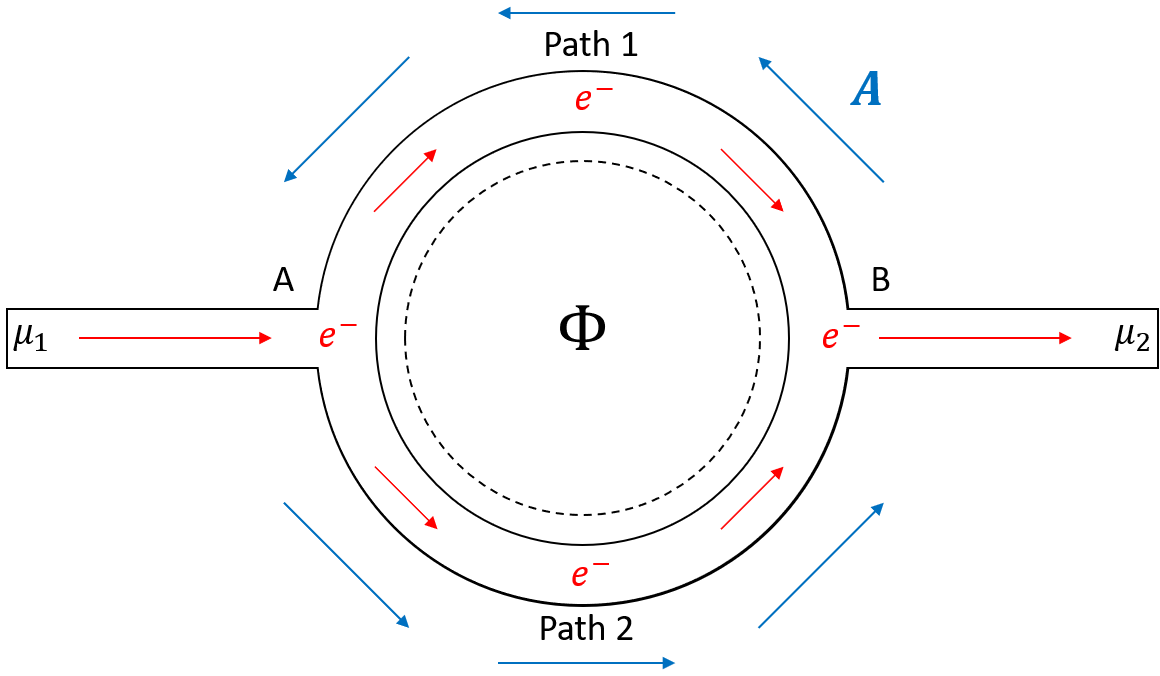
\includegraphics[scale=0.5]{ABEffectSolenoid.png}
    \caption{A diagram for a theoretical experiment to detect the A-B effect. The dotted circle is a cross section for a long solenoid with flux $\Phi$ and vector potential $A$, represented in blue with the direction of the field given by arrows pointing counter-clockwise, running tangential to the solenoid. The outer ring, with input and output, are an electron beam (wire) with two possible paths labelled 1 and 2, and a potential difference between the ends of the wire. The flow of electrons is given by red arrows, and the points A and B represent opposite ends of the loop around the solenoid.}
    \label{fig:solenoid}
\end{figure}

To understand the example, it is important to first understand two different definitions of momentum. The first is canonical momentum, $\mathbf{p}$, and is defined by the operator
\begin{equation}
    \hat{\mathbf{p}}=-i\hbar\nabla.
    \label{eq:canon}
\end{equation}
The second is kinematic momentum, $\mathbf{k}$, which is used to calculate the kinetic energy of a particle and is given by
\begin{equation}
    \hbar\mathbf{k}=m\mathbf{v}=\mathbf{p}-q\mathbf{A}
    \label{kinetic}
\end{equation}
where $m$ is the mass of the particle, $\mathbf{v}$ is it's velocity and $q$ is it's charge. A general wavefunction can be expressed as
\begin{equation}
    \psi=\psi_0\exp[\frac{i}{\hbar}(\mathbf{p}\cdot\mathbf{r}-Et)]=\psi_0\exp(-i\frac{Et}{\hbar})\exp(i\frac{\mathbf{p}\cdot\mathbf{r}}{\hbar})
\end{equation}
where $E$ is energy, $t$ is time and $\mathbf{r}$ is position. The powers of the exponential factors give the phase of the wavefunction.

Consider now the setup shown in Figure \ref{fig:solenoid}. From Equation \eqref{eq:canon}, the canonical momentum of an electron in the beam is given by
\begin{equation}
    \mathbf{p}=\hbar\mathbf{k}-e\mathbf{A}
\end{equation}
where $q$ is replaced with the charge of an electron, $-e$. Since energy is conserved in the experiment, $|\hbar\mathbf{k}|$ is constant and the phase of the wavefunction is given by
\begin{equation}
    S=-\frac{e}{\hbar}\mathbf{A}
\end{equation}
and by extension, the phase shift from A to B is
\begin{equation}
    \Delta S=-\frac{e}{\hbar}\int_A^B\mathbf{A}\cdot d\mathbf{l}.
\end{equation}
The relative phase shift on an electron can then be calculated by considering the phase shift around the entire loop. Assuming paths 1 and 2 are identical and running clockwise this this phase shift is calculated to be
\begin{equation}
    \hbar\Delta S_\text{rel}=-e\left(\int_1\mathbf{A}\cdot d\mathbf{l}-\int_2\mathbf{A}\cdot d\mathbf{l}\right)=-e\oint\mathbf{A}\cdot d\mathbf{l}.
\end{equation}
However, it can be shown by use of Stoke's theorem that the final integral is just equal to the enclosed flux, thus
\begin{equation}
    \hbar\Delta S_\text{rel}=-e\Phi.
\end{equation}

If the independent transmission amplitudes for path 1 and 2 are $a_1$ and $a_2$ respectively, then probability of transmission for an electron going from A to B is
\begin{equation}
    |a_1+a_2\exp\left(i\frac{e}{\hbar}\oint\mathbf{A}\cdot d\mathbf{l}\right)|^2=|a_1|^2+|a_2|^2+2|a_1||a_2|cos(2\pi\Phi/(h/e))
\end{equation}
where the final term is an interference term, suggesting that the transmission probability oscillates with magnetic flux with period $h/e$. If an electron is transmitted then backscattered back to A, the relative phase difference is now $2e\Phi$ and the period of the oscillations is $h/2e$.

\end{document}
